%%%%%%%%%%%%%%%%%%%%%%%%%%%%%%%%%%%%%%%%%%%%%%%%%%%%%%%%%%%%%%%%

% IEEEconf.cls file must exist in the same directory as the TeX file you want to compile
\documentclass[letterpaper, 10 pt, conference]{IEEEconf}

\title{\LARGE \bf
Computer History:\\Integrated Circuits
}
%why is the first email the only one that is small?
\author{Guillmer Germino\\Kenji Helms\\Jordan Medina\\
\small guillmer.germino@student.nmt.edu\\
\small kenji.helms@student.nmt.edu\\
\small jordan.medina@student.nmt.edu\\
\small {October 2020}
}

% Image/graphics support
\usepackage{graphicx} % takes care of graphic
\graphicspath{ {./images/} } %full file path to the images

% Formatting for lists
\usepackage{enumitem}

% Formatting for media
\usepackage{float}
\restylefloat{table}
\restylefloat{figure}
\usepackage[utf8]{inputenc}
\usepackage{epigraph}
\usepackage{graphicx}
\usepackage{caption}

\begin{document}


\maketitle

%%%%%%%%%%%%%%%%%%%%%%%%%%%%%%%%%%%%%%%%%%%%%%%%%%%%%%%%%%%%%%%%%%%%%%%%%%%%%%%%
\section{\underline{Introduction}\\\\
\small {\underline{The Confluence of Hardware and Software}}}
%maybe write more about how abstract processes are carried out by physical circuitry/ logical gates
The road from logic to physical computational devices winds through mechanical engineering, electrodynamics, and pure mathematics. The most fundamental mathematical operations within basic logic can be translated to an arbitrary number of physical forms of nearly any  variety. Utility, however, lies in discovering how to reliably produce user-friendly, stable forms for carrying out such tasks. Integrated circuits, devices at the heart of modern electronic computation, stand at the pinnacle of this technological challenge, and combine size, efficiency, and raw computational power. Though, in essence, they perform the same fundamental tasks as the most rudimentary forms of logical processors, integrated circuits represent a mastery over physical obstacles which allow the blisteringly rapid speed of modern digital life.


\section{History}
\subsection{Ambitious Beginnings}

As early as 1842, the vast potential of computation was known to the prescient minds of Augusta Ada and Charles Babbage. After working on his Difference Engine, Babbage's Analytical Engine took on the task of performing programmable calculations. With the careful help of Ada (commonly known as Ada Lovelace), the Analytical Engine was designed to: receive punch cards for initiating user input, store memory within the state of its mechanical wheels, perform the calculation of arithmetic operation, and return output in the form of punch cards and bells rings. 

\begin{figure}[h!]
\centering
\captionsetup{justification=centering}
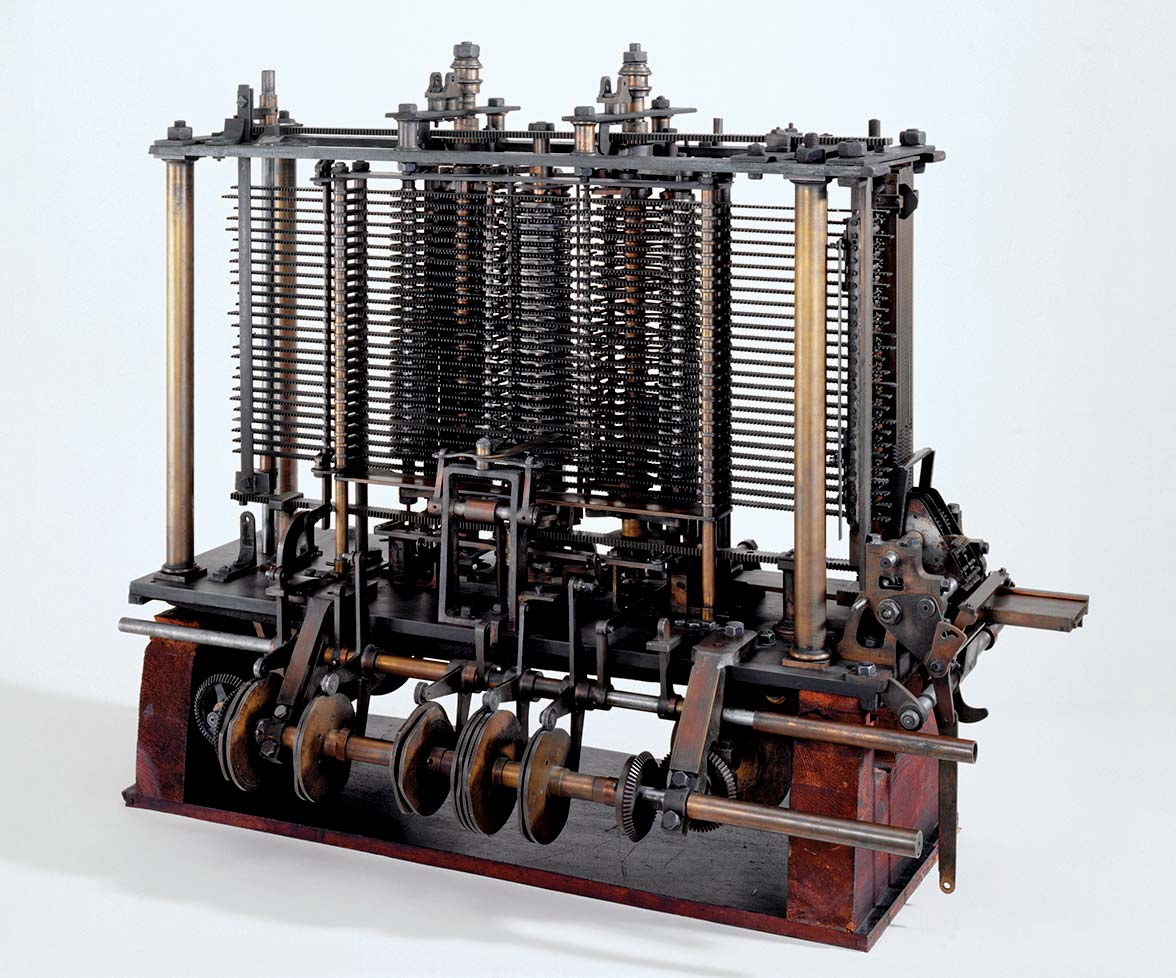
\includegraphics[width=0.4\textwidth]{portion-Charles-Babbage-Analytical-Engine-death-mill-1871.jpg}
\caption{The first general purpose computer, the Analytical Engine}
\label{fig:example}
\end{figure} 

In this form of the "computer," it is the relatively large components of mechanical gears and pegs which instantiate the logic of the underlying mathematics. Without a hint of modern electronic technology, logically meaningful instruction was stored in the macroscopic states of the wheels, which allow for the processing of input to output via mathematical rules. This incredible device was unfortunately left unfinished, but its design proved to be Turing-complete, essentially deeming the Analytic Engine as a true computer; an astonishing achievement for Victorian Age technology. 

\subsection{Vacuum Tube Technology}
With the prevalence of electricity-driven technology in the 20th century, it became possible to perform logical operations with the help of electronic components. Unlike the mechanically operated wheels of the Analytic Engine, electronic circuits allow for several orders-of-magnitude faster communications between hardware components. Vacuum tubes, along with their contemporaries, relay switches, are capable of storing memory states with the aid of electrical energy. Rather than storing the state of a logical operation in traditional physical form, vacuum tubes are advantageous for holding electrical energy, which can be received and transmitted almost instantly. 


\begin{figure}[h!]
\centering
\captionsetup{justification=centering}
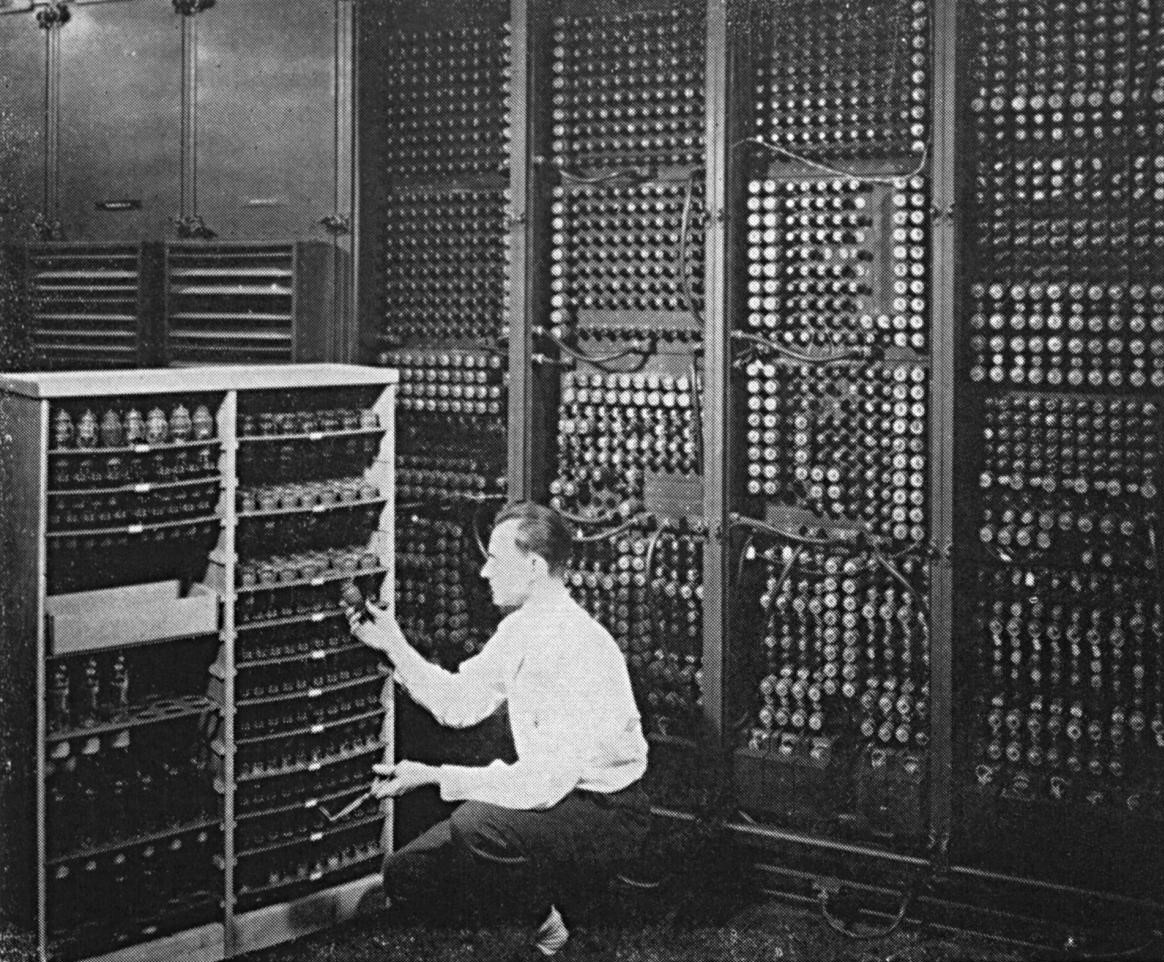
\includegraphics[width=0.4\textwidth]{ENIAC-changing_a_tube.jpg}
\caption{A technician changes a vacuum tube in the ENIAC}
\label{fig:example}
\end{figure}


%Talk about the timeline from vacuum tube, 

\section{Integrated Circuit Revolution}

While vacuum tubes were a revolutionary change in the history of computer hardware and made electronic computing possible for the first time, they also had major flaws that limited the capabilities of devices that relied on them. Vacuum tubes are very hot, large in size, and use a lot of electricity. The ENIAC needed over 17,000 vacuum tubes to work in one discrete component. In 1947, transistors were becoming available and being integrated into computers. Transistors had several advantages over vacuum tubes, but they had to be built one at a time and wired together manually to create a discrete component. To fix these flaws, Jack Kilby and Robert Noyce both independently created a new and reliable way of controlling electricity with the invention of integrated circuits in 1958. At the start of the 1960s, an integrated circuit (IC) was an assembly of an electronic circuit formed with 5 transistors on a single IC within a few square millimeters . Using photolithography and following Moore’s law, integrated circuits evolved into hundreds or thousands of transistors, and even resistors and capacitors were integrated. They could function like vacuum tubes, but also as an oscillator, a timer, a microprocessor, or even computer memory. The resulting circuits, integrated onto one piece of material, were better than vacuum tubes in size, voltage output, heat, and durability.


\begin{figure}[h!]
\centering
\captionsetup{justification=centering}
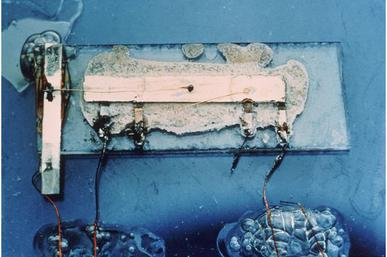
\includegraphics[width=0.4\textwidth]{Kilby_solid_circuit.jpg}
\caption{A picture of the original integrated circuit that Jack Kilby made in 1958}
\label{fig:example}
\end{figure}


\subsection{Cost/Efficiency}
Although integrated circuits tackle most of the problems vacuum tubes faced, integrated circuits still have some limitations. Because integrated circuits are fixed, the whole integrated circuit must be replaced in its entirety if a component is damaged, unlike a discrete circuit where a single component can be replaced easily. It also can only handle a limited amount of power, with the power dissipation being limited to 10 watts. 

\subsection{Moore's Law}
Integrated Circuits have gone through an immense growth per physical size over the years, leading to many of the breakthroughs enjoyed in modern technology. Starting in 1965, Gordon E. Moore, the co-founder of Intel noticed a trend in the number of transistors in an integrated circuit every two years. Moore’s law states that as every two years pass, the number of transistors on a chip doubles, while the cost of these chips is halved. Although this trend is supposed to be just a prediction, in later years it became a driving force for the electronics industry to follow. Whether unintentionally or deliberately, Moore's law has remained true for decades now, especially as innovations in computer technology continue to push forward.


\begin{figure}[h!]
\centering
\captionsetup{justification=centering}
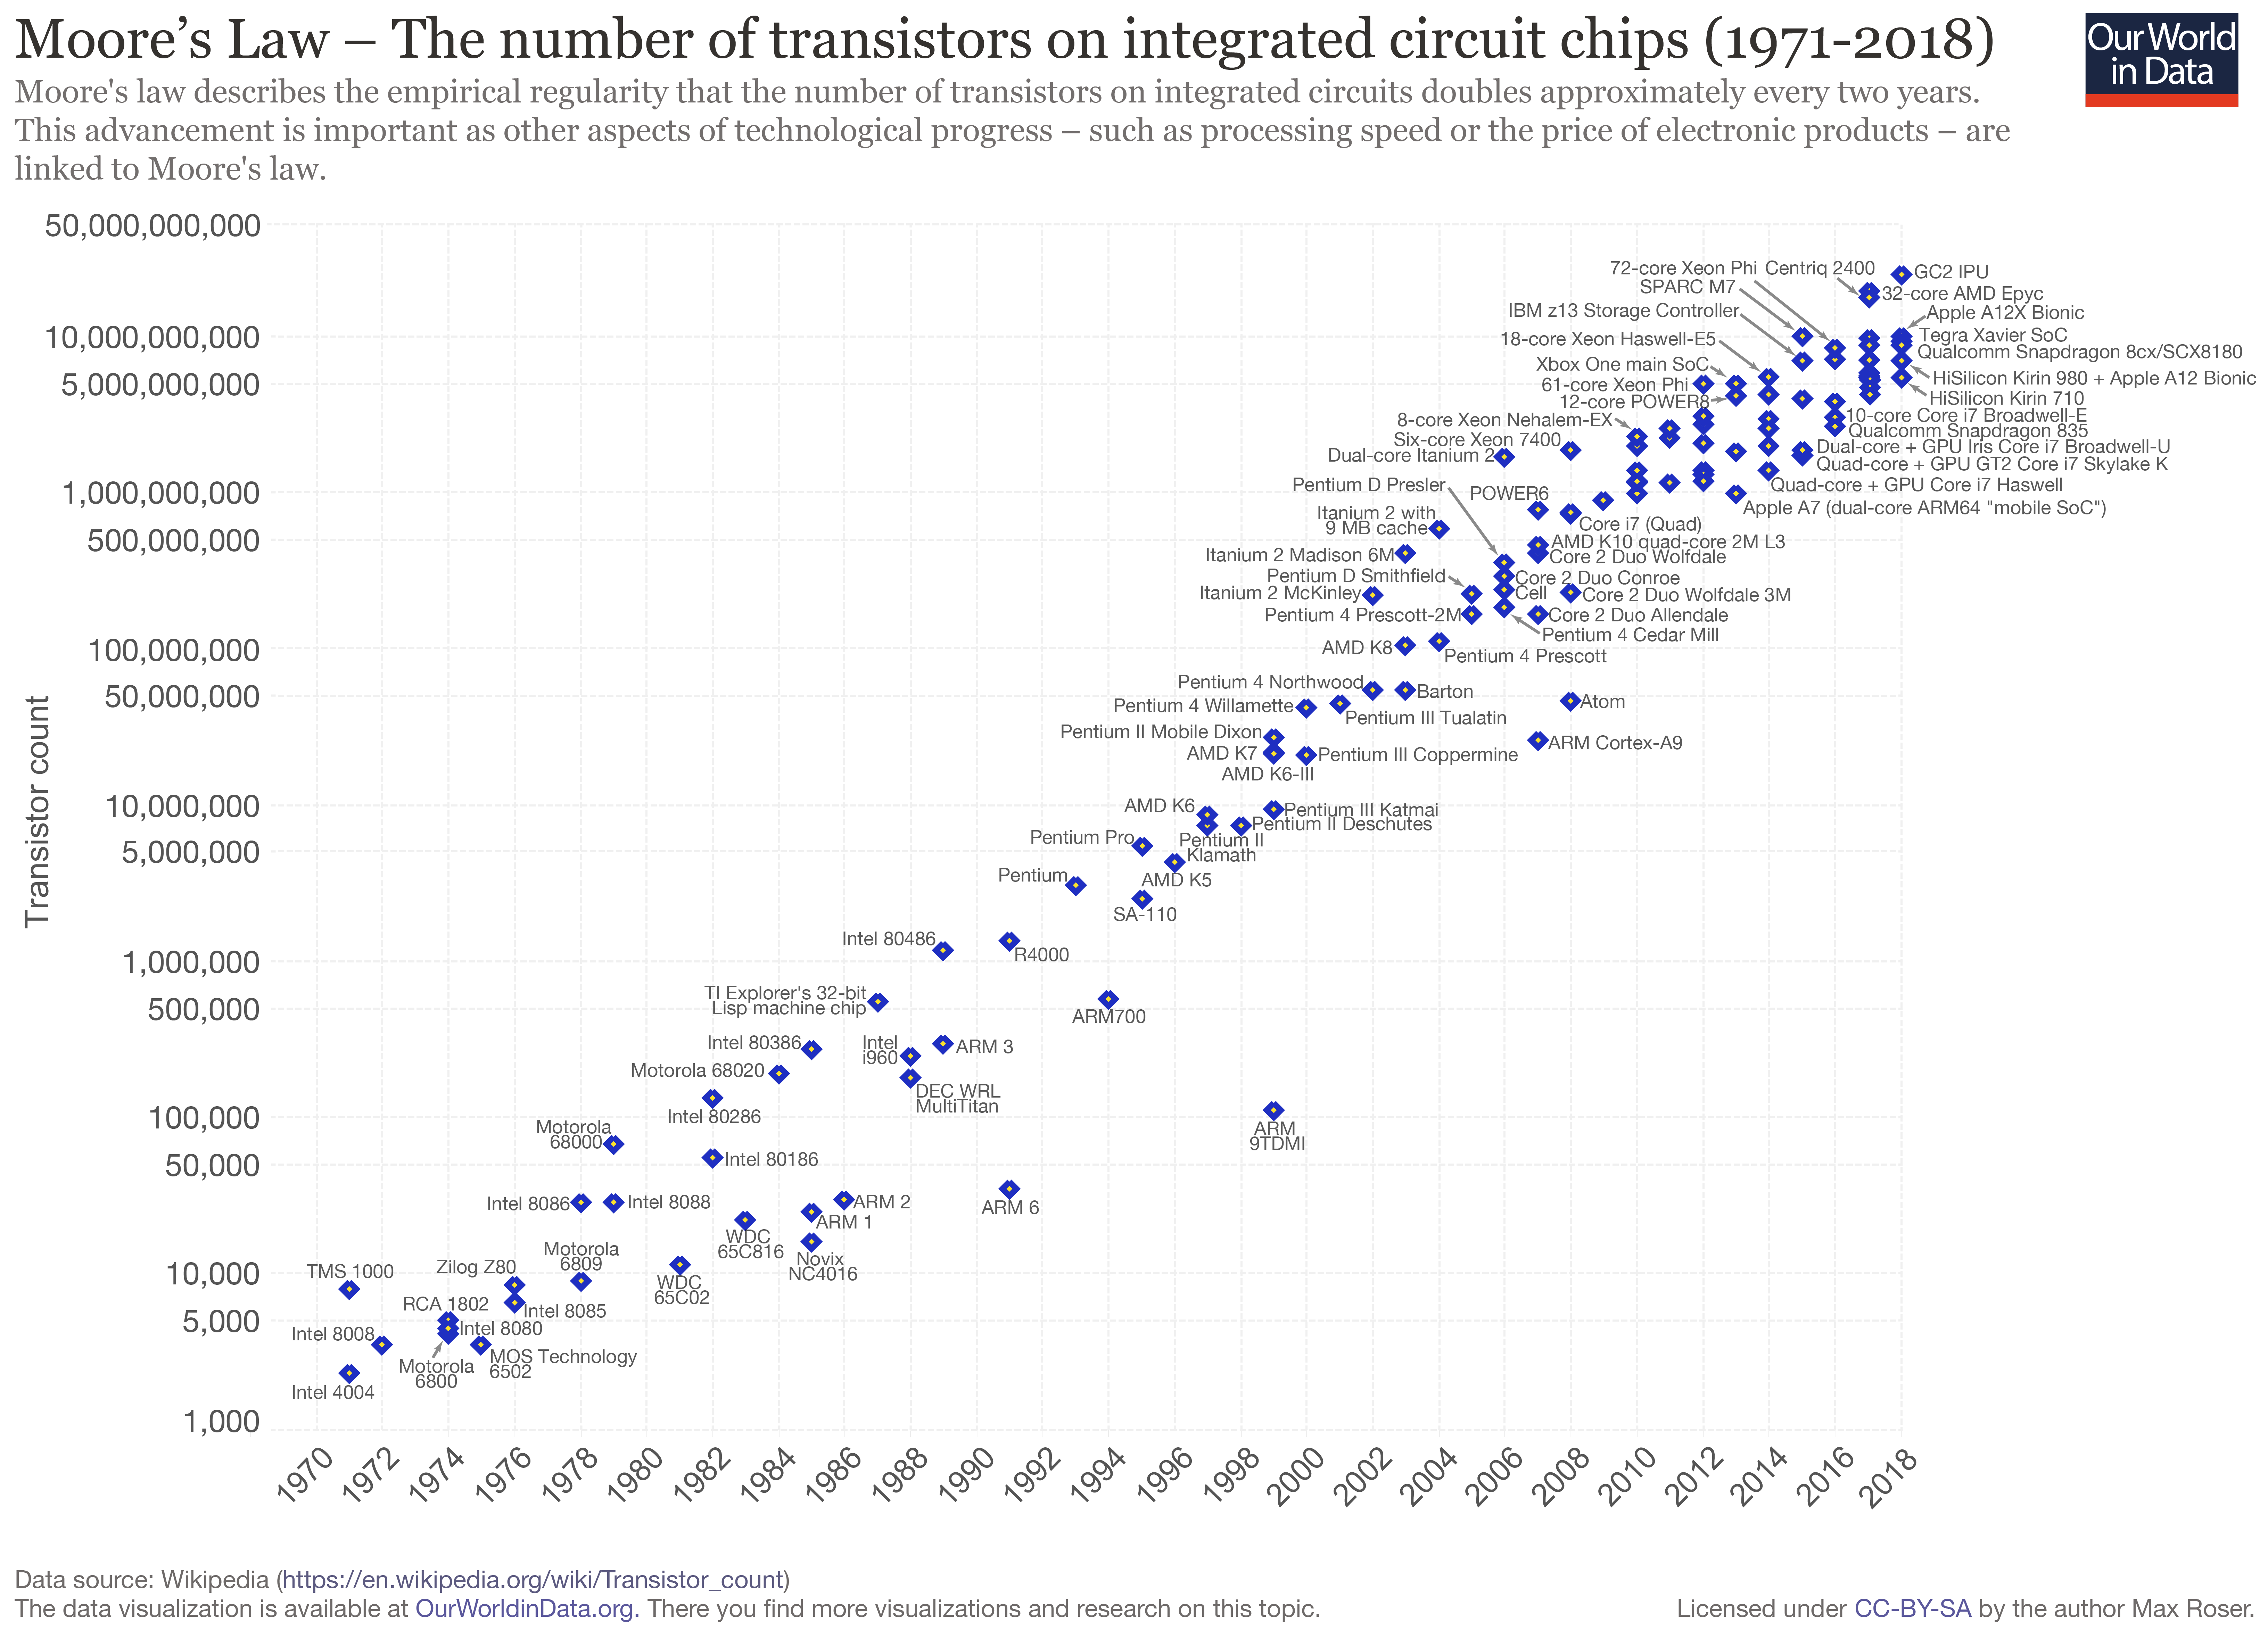
\includegraphics[width=0.4\textwidth]{Moore's_Law_Transistor_Count_1971-2018.png}
\caption{Integrated Circuit complexity over time, 1970-2018}
\label{fig:example}
\end{figure}


\section{CONCLUSION}

Modern computing technology is a field that continues to grow at amazing rates, but it is important to gain an understanding of the fundamental concepts that make up the technology we use today. Integrated circuits were clearly a major breakthrough in the history of computing, and therefore a great example of such a concept. Evolving from the need to store information for electronic computing, integrated circuits filled this role and grew to fill many more. Although it is impossible to define one concept that led to what people recognize as "modern computing," integrated circuits are certainly an essential stepping stone along the everlasting path of computer technology.

\section*{REFERENCES}


\begin{enumerate}[label={[\arabic*]}]
\item Rosen, Kenneth  H. Discrete Mathematics and Its Applications (Seventh Edition). McGraw-Hill, 2012. 
\item Woodford, Chris. “How Do Integrated Circuits Work?” Explain That Stuff, 30 Jan. 2020, www.explainthatstuff.com/integratedcircuits.html. 
\item Anysilicon. “The History of Integrated Circuit” anysilicon, 27 March, 2020, www.anysilicon.com/history-integrated-circuit.
\item “What is an Integrated Circuit (IC): Theory, Types of Integrated Circuits (Chips)” 27 February, 2010. Retrieved from https://www.brighthubengineering.com.


\end{enumerate}

\end{document}

